\documentclass[11pt,journal,transmag,final]{IEEEtran}

\usepackage{graphicx}
\usepackage{listings}
\usepackage{makecell}
\usepackage{hyperref}

\begin{document}

\title{Collective Report A}
\author{
    \IEEEauthorblockA{Daniel Carl Jones,}
    \IEEEauthorblockA{Department of Computer Science, University of Sheffield.}
    \IEEEauthorblockA{\today{}.}
}

\maketitle

\section{Introduction}

This report explores the results from applying PCA and Unsupervised Competitive Learning to a subset of the MNIST database\footnote{http://yann.lecun.com/exdb/mnist/} of hand-written letters.

The programmes presenting the results are implemented in Python\footnote{https://www.python.org/}. They utilise two main libraries: NumPy\footnote{http://www.numpy.org/} is used for linear algebra and maths; MatPlotLib\footnote{https://matplotlib.org/} is used to create graphs and visualsations in order to demonstrate the results.

The data provided are 28 by 28 pixel images of handwritten digits. The images are flattened as 784 dimensional feature vectors. The value for each pixel is a float representing simple greyscale intensity in the range 0 to 1.

\section{Principal Component Analysis}


Principal component analysis is a technique often used in dimensionality reduction. It is a technique used which rotates the data set into a new 'orthonormal coordinate system' with the least correlation and most variation per principal component \cite{eigenfaces}.

This report determines the principal components among the MNIST data set provided and compares some of the first few principal components.

\subsection{Algorithm}

The algorithm employed in this report is as follows:

\begin{enumerate}
    \item Centre or 'zero-mean' the data, as in equation \ref{eq:zero-mean}.
    \begin{equation}
        X_0 = X - \bar{X}
        \label{eq:zero-mean}
    \end{equation}
    \item Calculate the covariance matrix, as in equation \ref{eq:covariance}.
    \begin{equation}
        \textbf{C} = \textbf{X} \textbf{X}^T
        \label{eq:covariance}
    \end{equation}
    \item Calculate the eigenvalue-eigenvector pairs, using NumPy.
    \item Take each eigenvector in order of decreasing eigenvalue to create a feature transformation matrix.
    \item Multiply the centred data by the transformation matrix, creating the new transformed data set. This is shown in equation \ref{eq:tranform-data-set}, where $\textbf{F}$ is the feature transformation matrix.
    \begin{equation}
        \textbf{Y} = \textbf{X}_0 \textbf{F}
        \label{eq:tranform-data-set}
    \end{equation}
\end{enumerate}

This new data's dimensionality represents the principal components in decreasing order. By selecting a subset of the eigenvectors, the dimensionality can be reduced however for the purpose of this report, all dimensions are kept and a select few compared.

See code listing \ref{code:pca} for the Python implementation. A more detailed implementation is included seperately.

\subsection{Comparison of Principal Components}

Figure \ref{fig:pca-results} shows the results of the principal component analysis of the reduced MNIST data set. Five graphs are plotted with different components selected on different axes.

Only five numbers (0,1,4,6,7) have been plotted to ensure clarity and ease of comparison. It should however be noted that other numbers may overlap with the clusters shown.

Each cluster is plotted in three dimensional space, each of the dimensions labelled on the axes. The clusters are colour coded by the training labels provided, and the mean or centre of the clusters is labelled too.

\begin{figure*}[!t]
    \begin{center}
        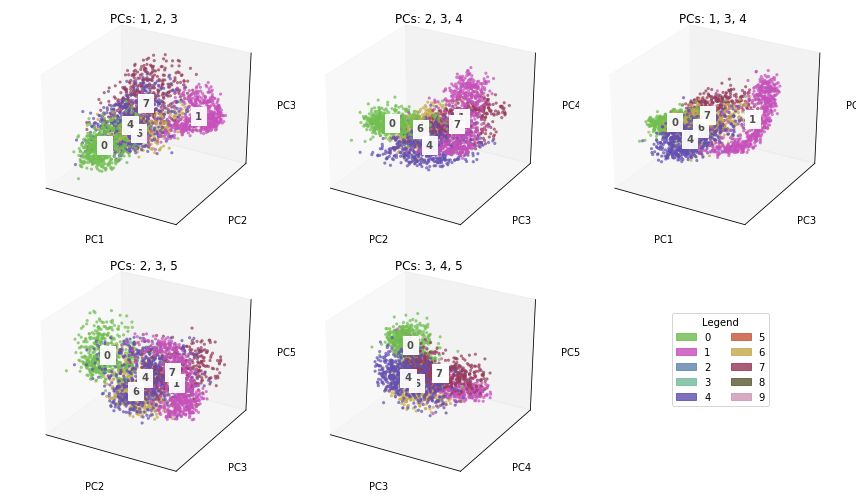
\includegraphics[width=\textwidth,keepaspectratio]{figures/pca-results.png}
        \caption{Principal Component Analysis of a subset of the MNIST Database}
        \label{fig:pca-results}
    \end{center}
\end{figure*}

In the graph with PCs 1, 2, and 3, the clusters are fairly seperated --- it is possible to spot each of the five cluster centres. Despite the data originally consisting of 784 different data points representing each pixel (28x28), it is possible to select three data points and begin to differentiate between each number. Issues begin to arise when numbers 4 and 6 are compared. The labels show the cluster centres in a similar position meaning that there is little variation when comparing the three components.

While it isn't possible to seperate the numbers with just three components, it illustrates the power behind PCA. The more components being retained will allow for better comparison.

Comparing all of the plots, the first showing PCs 1, 2, and 3 are the most meaningful. This plot appears to have the least correlation among cluster centres. In all the others, at least two pairs of cluster centres overlap. In plot PCs 3,4,5, the cluster centres for 1 and 7 are almost indistinguishable meaning that this combination would be useless for a system attempting to classify between 1 and 7.

\section{Competitive Learning}

This section explores unsupervised learning techniques in a single-layer feed-forward neural network. The network implements a hebbian learning rule and adapts the 'winner takes all' approach implementing a competitive network with 'leaky learning'. The aim of this network is not neccesarily to classify the numbers but instead to cluster inputs into a group or unit that is formed.

A series of weight vectors will be produced which may bear resembelance to cluster centres --- since this is effectively what they are. As this is unsupervised learning, it is difficult to get ten perfect clusters representing each number. Some clusters may be duplicated whereas others may not be detected, hence a greater number of output units will be produced with each number represented.

\subsection{Algorithm}

The algorithm employed for competitve learning in this report is as follows:

\begin{enumerate}
    \item Load and normalise the unlabelled data, initialise and normalised weight matrix.
    \item Select a random input sample, compute the postsynaptic frequencies using equation \ref{eq:postsynaptic-calc} or \ref{eq:postsynaptic-calc-vec}.
    \begin{equation}
        y_i = \sum_j w_{i, j}x_j
        \label{eq:postsynaptic-calc}
    \end{equation}
    \begin{equation}
        \textbf{y} = \textbf{W}\textbf{x}^{T}
        \label{eq:postsynaptic-calc-vec}
    \end{equation}
    \item If applicable, apply any noise or rotation to the input smaple selected.
    \item Determine the winning neuron using \textit{NumPy.max} on the postsynaptic outputs.
    \item Calculate the weight change for this neuron and add it to the neuron's weight vector. The weight change is calculated using the simple competitive learning rule --- see equation \ref{eq:simple-competitive-rule}. $\eta$ is the learning rate.
    \begin{equation}
        \Delta \textbf{w}_{i} = \eta (\textbf{x} - \textbf{w}_{i})
        \label{eq:simple-competitive-rule}
    \end{equation}
    \item Apply a scaled down version of this weight change to the non-winning neurons. Leaky learning.
    \item Repeats steps 2-5 for a number of iterations until the weight change becomes negligible and the system has converged. 
\end{enumerate}

This algorithm is 'online', meaning that the latest value of the weights are used in the calculation for postsynaptic frequencies and weight updates. Batch is where a selection of input patterns are processed and the weight change is only applied at the end of the batch. Once the weight is updated, more batches are often processed. The algorithm in this report has an effective batch size of 1.

See code listing \ref{code:nn} for the Python implementation. A more detailed implementation is included seperately.

\subsection{Normalisation of Vectors}

The training data and initial weight vectors are both normalised to unit length --- in other words, the euclidean distance of the vector is 1. This is important to ensure that input data is not extreme and prevent a sample from dominating a network.

\begin{equation}
    \Delta \textbf{W} = \eta \textbf{x} \textbf{y}^{T}
    \label{eq:hebb-rule}
\end{equation}

The weight vectors are also normalised.

The basic hebbian rule, equation \ref{eq:hebb-rule}, simply takes the product of the presynaptic and postsynaptic frequencies. The problem with this rule is that the weights are unbounded. After each pattern seen, the network will increase the weights assuming the frequencies are always positive. This becomes an issue when one particular pattern dominates the network and will result in a particular neuron with strong weights always firing.

In the bounded learning rule, the weight change is calculated using the presynaptic frequencies $\textbf{x}$, and then subtracting the current weight vector $\textbf{w}_i$. By subtracting the weights in this way, they can be prevented from growing without bounds. The larger the weight, the larger the amount subtracted from the weight change, becoming negative if the input frequency is small enough.

\subsection{Improvements on Simple Competitive Learning}

\begin{equation}
    Purity = \frac{1}{N} \sum_{i=1}^{k} max_j | c_i \cap t_j |
    \label{eq:purity}
\end{equation}

Table \ref{table:nn} shows some metrics measured against the neural network with different optimisations applied. Each value measured was calculated by taking the mean from 50 test runs of the neural network generating new prototypes each time.

Dead units is simply the dead unit count as explained in section \ref{section:nn:dead-unit-identification}. Another metric used in this report to measure optimisations is Cluster Purity, shown in equation \ref{eq:purity}\cite{clusterAnalysis}. This measure is only possible to calculate with data where the testing data is labelled --- labelled data is not usually available for unsupervised learning, and so this score can only be used to evaluate the techniques used to optimise the network.

It is also important to acknowledge that the networks can be quite volatile and --- time permitting --- it would have been better to calculate the metrics over a much larger series of test runs.

\begin{table}
    \centering
    \caption{Optimisations of the Neural Network}
    \label{table:nn}
    \begin{tabular}{l|lllll}
    & Basic & Noise & \makecell{Leaky \\Learning} & Rotation & All \\
    Dead Units & 5.52 & 5.14 & 5.56 & 5.2 & 6.50 \\
    Cluster Purity & 0.639 & 0.668 & 0.670 & 0.651 & 0.644
    \end{tabular}
\end{table}

\subsubsection{Presynaptic Noise}

By adding a small amount of noise to the calculation, it allowed units which may otherwise have never activated to win and update their weight towards the input. It helps generalise the prototypes such that new unseen inputs may be appopriately clustered with related data. The noise applied in this report were values between 0 and 0.005 --- a small fraction compared to the maximum value for each pixel.

Looking at the metrics in table \ref{table:nn}, we see that the dead units decrease and the purity of the clusters has increased. Adding noise actually results in the best improvements to both the quantity of dead units and the cluster purity.

\subsubsection{Leaky Learning}

Leaky learning is an alternative to the 'winner takes all' approach. Instead of only updating the weight of the winning prototype, all prototypes get updated. The winning prototype gets a full weight update as in equation \ref{eq:simple-competitive-rule}, whereas the losing prototypes get updated with a reduced learning rate. In this report, the reduced learning rate was 0.1\% of the learning rate $\eta$, where $\eta = 0.09$.

Leaky learning implemented in this way appeared to show improvement according to the cluster purity metric, but not the dead unit count. This would indicate that while there are now more dead units, the clustering of each number is now better.

\subsubsection{Rotation}

The final optimisation applied to the network is rotation of the input image. The feature vector is reshaped to the actual 28 by 28 pixel image is represents, rotated by a random amount up to $\pm5^{\circ}$. The improvements are justified in a similar way to presynaptic noise. By rotating the input slightly, it should help to generalise the prototypes. An example with this dataset would be how the number 1 will often generate two prototypes. This is because with repect to the feature vector, a 1 perfectly vertical would look entirely different to a 1 that is at a slight angle which is a common occurance with handwriting.

The addition of rotation saw an improvement to both the dead unit count and cluster purity. The cluster purity improvement was only marginal, and it did result in strange looking prototypes. Instead of being clear digits, they had a ghosting effect around them.

Several angles were trialed before finding $\pm5^\circ$ as the optimal one. These are listed in table \ref{table:nn-rotations}.

\begin{table}[h]
    \centering
    \caption{Dead Units by Maximum Rotation Angle}
    \label{table:nn-rotations}
    \begin{tabular}{l|llll}
                    Rotation & $\pm20^\circ$ & $\pm10^\circ$ & $\pm5^\circ$ & $\pm2.5^\circ$ \\
                    Dead Units & 5.56 & 5.62 & 5.20 & 5.48
    \end{tabular}
\end{table}

While inapproriate for a generalisation of unsupervised learning, it is interesting to note that when rotating the inputs only by a clockwise amount only (no counter-clockwise rotation), the metrics saw a small improvement in dead units scoring 5.18. This could be explained by considering the way many people handwrite letters and digits at an angle to the paper, often resulting in more italisised characters.

\subsubsection{Combining All The Optimisations}

By combining all the optimisations, it would be expected to see a larger improvement in the metrics. Dead units increased which, given the large influence leaky learning had on the value, should be expected. However, cluster purity also increased which I would describe as being an overall improvement.

Dead units are not useful but so long as we have enough clusters to represent the classes, they can be ignored and removed. If this is the case, the output of the network has improved for the clusters.

\subsection{Dead Unit Identification}
\label{section:nn:dead-unit-identification}

In this report, a simple method of dead unit identification is used. Any unit that wins less than 2\% of the time is identified as dead. In practice, this measure has been adequate but leaves much to be desired. A limitation of this method is that it does not take into account units which are very similar to one another resulting in the wins being split among them.

\subsection{Weight Change Over Time}

\begin{figure}[b]
    \begin{center}
        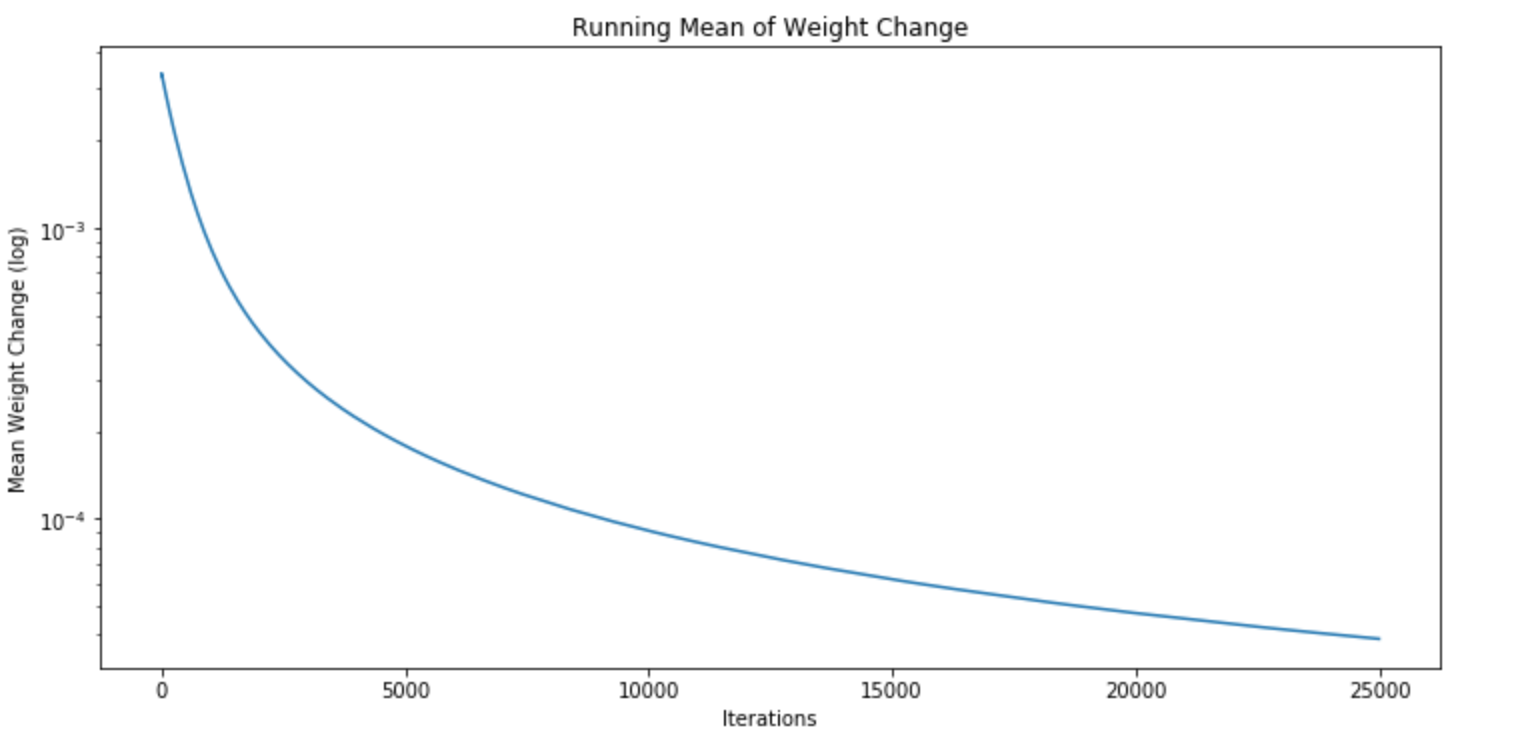
\includegraphics[width=\linewidth,keepaspectratio]{figures/nn-weight-change.png}
        \caption{Mean Weight Change Over Time}
        \label{fig:nn-mean-weight-change}
    \end{center}
\end{figure}

Since the algorithm is 'online', it is possible to record the average weight change each iteration. This can be plotted as a smooth curve as in figure \ref{fig:nn-mean-weight-change}. The y-axis is on a logarithmic scale.

From the graph, it is possible to identify where there is no longer much point in continuing learning, since the weight change approaches a constant change indicating oscillation. Within the first approximately 2500 iterations, the mean weight change has already dropped by 1 order of magnitude. This means that the weight change is now 10 times smaller. As the iterations increase, the weight change continues to approach a stable value. It may not be worth running the network for the 25000 iterations shown, however it has been included for completeness.

\subsection{Prototypes}

\begin{figure}[!t]
    \begin{center}
        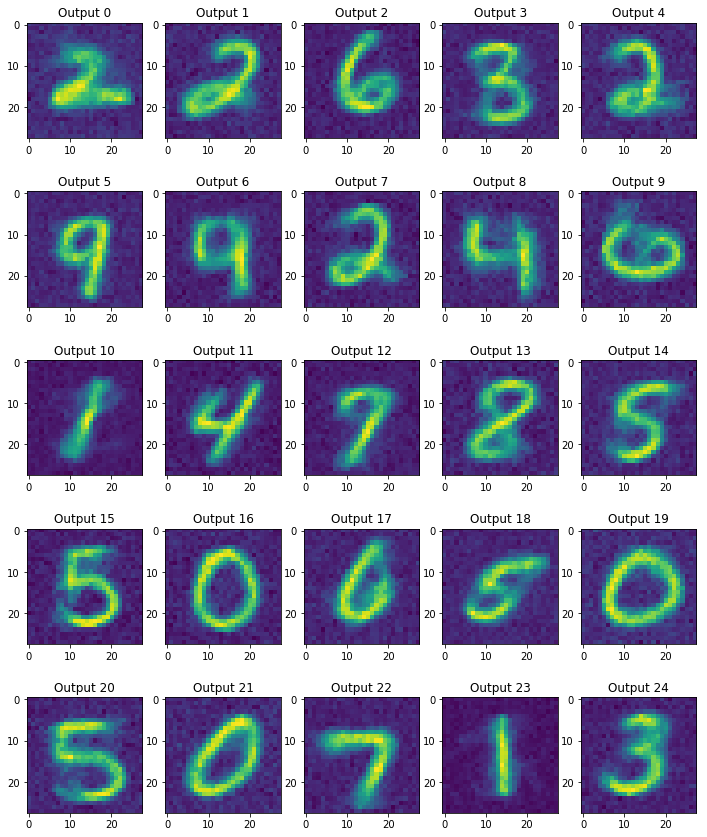
\includegraphics[width=\linewidth,keepaspectratio]{figures/nn-results.png}
        \caption{Prototypes Output From Competitive Learning}
        \label{fig:nn-prototypes}
    \end{center}
\end{figure}

Figure \ref{fig:nn-prototypes} shows the prototypes output from the neural network. These prototypes represent the weight vectors for each postsynaptic neuron, reshaped back into a 28x28 pixel image. The numbers are quite easily recognisable in most of the prototypes.

These prototypes represent the centre for each cluster. The calculation of post-synaptic frequencies as in equation \ref{eq:postsynaptic-calc} can be likened to a distance calculation of the input vector from the cluster centre.

Some of the prototypes could be considered dead or a mixture of two clusters. For example, output 9 looks very much like both a 0 and a 6. Meanwhile, output 19 represents the digit 0 and output 2 represents the digit 6.

Some duplicate clusters can be seen in the prototypes. For example, output 15 and 18 both represent the digit 5 but the latter is rotated clockwise by a small amount.

More assertions can be made using the correlation matrix (figure \ref{fig:nn-correlation}) in section \ref{section:nn:correlation}.

\subsection{Correlation Matrix Between Prototypes}
\label{section:nn:correlation}

To calculate the correlation, the program produces a matrix similar to a confusion matrix. This illustrates the frequency at which the neural network places a digit in a specific cluster. A graphical representation of the confusion matrix is shown in figure \ref{fig:nn-confusion}.

\begin{figure}
    \begin{center}
        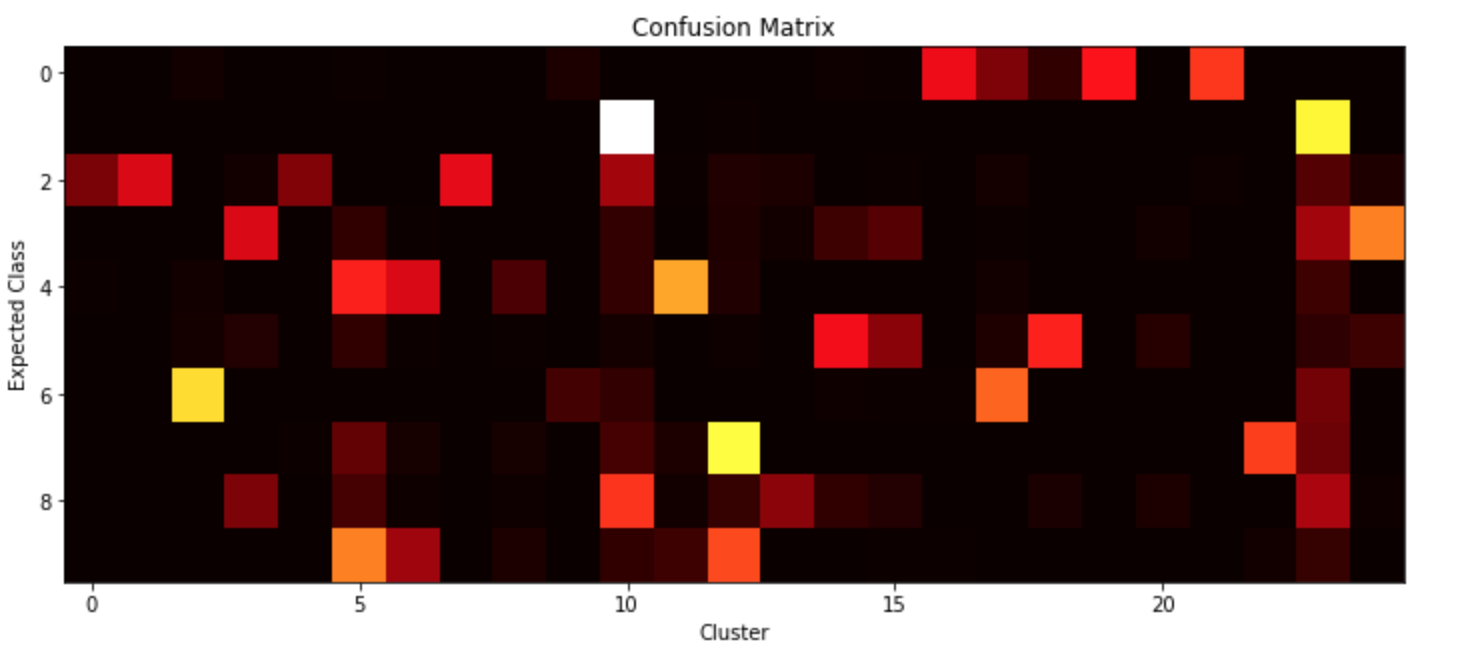
\includegraphics[width=\linewidth,keepaspectratio]{figures/nn-confusion.png}
        \caption{Confusion Matrix for the Prototypes}
        \label{fig:nn-confusion}
    \end{center}
\end{figure}

\begin{figure}
    \begin{center}
        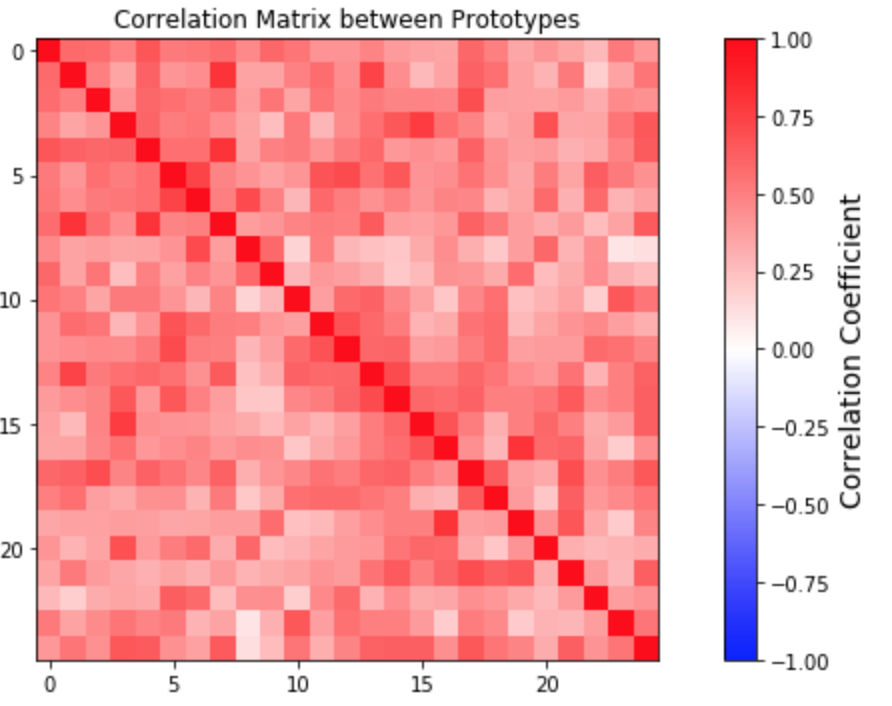
\includegraphics[width=\linewidth,keepaspectratio]{figures/nn-correlation.png}
        \caption{Correlation Matrix for the Prototypes}
        \label{fig:nn-correlation}
    \end{center}
\end{figure}

Figure \ref{fig:nn-correlation} shows the correlation matrix between the prototypes. The correlation matrix is based on the Pearson product-moment correlation coefficient. This produces a value between 1 --- where the two variables perfectly correlate --- and -1 --- where the two variables negatively correlate. A value of 0 indicates no correlation.

Given the nature of the images containing the number at the centre with no colour around the edges, the matrix on the whole is red showing a positive correlation. The greater the intensity of the red, the more closely the prototypes correlate.

Looking at the prototypes in figure \ref{fig:nn-prototypes}, prototype 8 shows the number 4 and 23 shows the number 1. The correlation matrix shows a low correlation value between the two prototypes. Meanwhile, prototypes 16 and 19 both represent the number 0. In the correlation matrix, the prototypes have a very high correlation coefficient. The red diagonal line shows the coefficient of each prototype with itself --- naturally, this is 1.

This tells us that it may be possible to combine prototypes if they show enough correlation.

\section{Using PCA and Competitive Learning Together}

Using PCA together with competitive learning could be used to improve results if applied carefully. Principal component analysis creates a new co-ordinate space and depending on which eigenvectors are selected, important dimensions could be lost. In this application, it could work quite well since many of the dimensions such as the outermost pixels in the image are not useful when comparing digits. By selecting the most variant principal components, it should allow the network to concentrate on the main differences between each digit and prevent overfitting.

\section{Reproducing The Results}

The code used to produce these results are included as two Jupyter Notebooks\footnote{http://jupyter.org/}. The graphs and results are taken from these projects.

If using an environment like Anaconda, the libraries should all be preinstalled and require no setup. Starting up a Jupyter server for the notebooks should be all that is required.

\onecolumn
    \begin{appendices}
        \section{Code Listings}

        This section contains simplified code listings for both algorithms. For full solutions, see the seperated Jupyter notebooks.

        \begin{lstlisting}[language=Python, caption=Principal Component Analysis Code, basicstyle=\footnotesize, label=code:pca]
# Assuming train is loaded with data...

# Take the mean of each feature for the training set
mean = np.mean(train, axis=1)
centered_data = train - mean[:, None]
cov_m = np.cov(centered_data, rowvar=True) # Covariance Matrix!

# Calc Eigenvectors & Eigenvalues
eig_vals_unsorted, eig_vecs_unsorted = np.linalg.eig(cov_m)

sorted_indices = np.argsort(eig_vals_unsorted)[::-1] # Find indices in dec order

eig_vals = np.real(eig_vals_unsorted[sorted_indices]) # Reorder eigenvalues
eig_vecs = np.real(eig_vecs_unsorted[sorted_indices]) # Reorder eigenvectors
    
new_data = np.dot(eig_vecs.T, centered_data) # Data in new transformed space
        \end{lstlisting}

        \begin{lstlisting}[language=Python, caption=Competitive Learning Code, basicstyle=\footnotesize, label=code:nn]
# Assuming raw_train is already populated...
train = preprocessing.normalize(raw_train, axis=0, norm='l1')

eta = 0.09; # learning rate
output_quantity = 25
iterations = 25000

# Optimisations
noise_max = 0 # 0.005
rotation_max = 10 # 5
leaky_learning_rate = 0 # 0.2

# Init W
W = preprocessing.normalize(np.random.rand(output_quantity, feature_size), axis=0, norm='l1')

def simple_competitive_rule(x, y, W, max_index):
    delta_W = np.ma.array(np.zeros(W.shape), mask=False)
    weight_change_vector = eta * (x.T - W[max_index])
    
    delta_W[max_index] = weight_change_vector
    
    delta_W.mask[max_index] = True
    delta_W += weight_change_vector * leaky_learning_rate
    
    return delta_W.data

# LEARN!
for t in range(iterations):
    i = math.ceil(num_samples * np.random.rand()) - 1 # Pick rand sample
    input_sample = deepcopy(train[:,i])
    
    if rotation_max != 0:
        rand = np.random.rand(1,1)
        rotation_angle = (np.random.rand(1,1) * rotation_max * 2) - rotation_max
        input_sample = np.reshape(input_sample, image_shape) # Reshape to the image
        # Rotate the image
        input_sample = scipy.ndimage.rotate(input_sample, rotation_angle, reshape=False)
        input_sample = np.reshape(input_sample, feature_size) # Back to a flat vector
        
    if noise_max != 0:
        input_sample += np.random.rand(feature_size) * noise_max # Add noise

    x = input_sample # Presynaptic
    y = np.dot(W, x) # Postsynaptic

    max_index = np.argmax(y) # Get winner
    winner_count[max_index] += 1 # Update winner count

    d_W = simple_competitive_rule(x, y, W, max_index) # Calculate delta W

    W += d_W # Update W
        \end{lstlisting}
    \end{appendices}


    \bibliography{assignment} 
    \bibliographystyle{IEEEtran}
\end{document}
